\documentclass[11pt,a4paper]{article}
\usepackage[utf8]{inputenc}
\usepackage[T1]{fontenc}
\usepackage[english]{babel}
\usepackage{lmodern,microtype}
\usepackage[margin=27mm,headheight=14pt]{geometry}
\usepackage{amsmath,amssymb,amsthm,mathtools}
\usepackage{booktabs,array,graphicx,caption,enumitem}
\usepackage[authoryear,round]{natbib}
\usepackage[colorlinks=true,linkcolor=black,citecolor=black,urlcolor=blue]{hyperref}
\hypersetup{pdftitle={Robust Fairness in Open Heterogeneous Tontines},
 pdfsubject={Scientific working paper, Version 1.0, English edition},
 pdfkeywords={Tontine, Longevity Pooling, Robust Fairness, Mortality Misspecification}}
\usepackage{fancyhdr}
\pagestyle{fancy}\fancyhf{}
\fancyhead[L]{\small Robust Fairness in Heterogeneous Tontines}
\fancyhead[R]{\small Working Paper}
\fancyfoot[C]{\thepage}
\setlength{\parskip}{4pt}
\setlength{\parindent}{12pt}
\setlength{\emergencystretch}{3em}
\setlist{itemsep=2pt,topsep=3pt}
\newtheorem{theorem}{Theorem}[section]
\newtheorem{lemma}[theorem]{Lemma}
\newtheorem{corollary}[theorem]{Corollary}
\newtheorem{proposition}[theorem]{Proposition}
\theoremstyle{definition}\newtheorem{definition}[theorem]{Definition}
\theoremstyle{remark}\newtheorem{remark}[theorem]{Remark}
\newcommand{\E}{\mathbb E}
\newcommand{\R}{\mathbb R}
\newcommand{\one}{\mathbf 1}
\newcommand{\diag}{\operatorname{diag}}
\newcommand{\pos}[1]{\left(#1\right)_+}
\newcommand{\calH}{\mathcal H}
\newcommand{\calF}{\mathcal F}
\newcommand{\calG}{\mathcal G}
\newcommand{\calI}{\mathcal I}
\title{Robust Fairness in Open Heterogeneous Tontines\\[5pt]
\large A Sharp Frontier for Mortality Pooling, Model Error and Death Benefits}
\author{}
\date{Scientific Working Paper, Version 1.0, English Edition\\2 October 2026}
\begin{document}
\maketitle
\begin{abstract}
We study fully funded open longevity pools with individual accounts, heterogeneous death intensities and voluntary exits. Within a class of nonnegative, locally balanced death-contingent transfers, we characterize the individual wealth transfers caused by unknown mortality misspecification. The misspecification drift equals the negative product of a weighted Laplacian matrix and the vector of relative intensity errors. Exact robust fairness requires identical error factors along every transfer edge; independently variable individual errors therefore rule out nontrivial pooling. For a rectangular uncertainty set with relative half-width $\varepsilon$, the worst-case individual drift is exactly $2\varepsilon d_i$, where $d_i$ denotes the modelled mortality-transfer exposure. Individual error tolerances $\delta_i$ induce capacities $b_i=\min(\mu_iA_i,\delta_i/(2\varepsilon))$. We prove that the minimum modelled death-benefit rate is $K-B+(2\max_i b_i-B)_+$ and construct an attaining rule. A martingale argument justifies exits at account value under correct public information; bounded misspecification yields a bound on information-dependent wealth transfers. We also explain why entry neutrality does not imply distributional neutrality and why necessary death benefits constrain globally constant expected payouts conditional on survival in this finite-pool model. Reproducible state checks and event-driven R simulations illustrate the proven results.
\end{abstract}
\noindent\textbf{Keywords:} Tontine; longevity pooling; robust actuarial fairness; mortality misspecification; death benefit; exit option; finite pool.\\
\textbf{Status:} AI-assisted research draft for expert review. The mathematical statements are proved below; scientific priority and readiness for publication are not claimed. Authorship and institutional affiliation have not yet been assigned.

\section{Introduction and Research Question}
Open tontines seek to let people of different ages and wealth levels participate in mortality credits without an external guarantor. Individual accounts make funding transparent. The central challenge is the valuation of the risks transferred among members: fairness under estimated survival probabilities does not ensure fairness under unknown actual probabilities.

This paper therefore asks: how much mortality pooling is possible when individual mortality assumptions may be wrong and the resulting expected wealth transfers must remain bounded? The objective is an explicit state-dependent construction. We maximize pooling volume subject to specified local fairness constraints; expected utility, income variance and a market price for guarantees are not the optimization objectives.

The main theorem combines two distinct constraints. First, unknown individual mortality limits admissible exposure. Second, a finite pool cannot transfer all of a dominant member's risk to the remaining members while preserving nonnegative, locally fair transfers. The two effects enter additively into a closed-form frontier. The formula is an exact optimal solution within the specified model class; its combination with the robustness requirement is the candidate contribution investigated here.

\subsection{Related Literature and Scope of the Contribution}
Fair heterogeneous transfer plans and their computational implementation are established topics. \citet{sabin2010,sabin2011} study fair tontines and transfer algorithms. \citet{fullmer2019} develop open individual tontine accounts. \citet{weinert2021} investigate a fair revolving tontine with heterogeneous personal characteristics and contributions. Their condition that no member holds more than half of the risk exposure is an important antecedent of our finite-pool capacity constraint. No novelty is claimed for this basic idea.

Death benefits and the choice of a pooling fraction are also established. \citet{bernhardt2019} combine tontine and bequest accounts; \citet{dagpunar2021} derives optimal controls for an ideal model with a bequest motive. Here the required retained fraction is instead determined by robust fairness constraints and finite membership. This is a different objective, rather than a refutation of those utility models.

For exits, \citet{weinert2017} is particularly relevant: fair surrender values are studied using expected values and payout volatility. The full text was unavailable during the literature review underlying this manuscript; the description relies on its bibliographic abstract and the discussion in \citet{weinert2021}. \citet{he2023} study reversible tontines as an impulse-control problem with transaction costs. Neither exit flexibility nor the mere combination of pooling and reversible accounts is therefore presented as a new contribution. \citet{butt2026} analyse flexible payouts and adverse selection; our local bound addresses a related question from a different mathematical perspective.

\citet{zhou2025} develop rules for stochastic and correlated mortality, including a joint-expectation rule. We instead impose a pointwise bound on misspecification-induced transfers for every intensity configuration in a specified uncertainty set. Correctly calibrated stochastic mortality and unknown model misspecification are distinct valuation problems.

Graph Laplacians are likewise not new to risk sharing: \citet{fogarty2026} investigate fair linear network rules and a connection to the graph Laplacian. Our potential contribution is the specific robustness frontier derived for finite mortality pools and its link to death benefits and stopping times. The reviewed sources establish related concepts; they establish neither exhaustive literature coverage nor priority for the statements formulated here.

\section{Model, Information and Fairness Concepts}\label{sec:model}
\subsection{Time, Membership and Accounts}
On a filtered probability space satisfying the usual conditions, $\calF_t$ denotes public information. Member $i$ enters at a stopping time $e_i$ with capital $C_i>0$. Their death time is $\tau_i>e_i$, and voluntary exit occurs at a stopping time $\sigma_i$. Active membership at time $t$ is
\[
\calI_t=\{i:e_i\le t<\tau_i\wedge\sigma_i\}.
\]
There are finitely many entries and transactions on each bounded time interval. Death events have no common jumps. Death intensities $\mu_i(t)$ are positive, predictable and locally integrable; in the basic model they are deterministic and individual residual lifetimes are independent. Entrants bring fully funded new accounts. New entries are not required to finance existing accounts.

The interest rate $r(t)$ is deterministic, and the discount factor is
\[
D(s,t)=\exp\left(-\int_s^t r(v)\,dv\right),\qquad D(t)=D(0,t).
\]
An active account $A_i(t)\ge0$ starts at $A_i(e_i)=C_i$. Between events,
\begin{equation}\label{eq:accountflow}
dA_i(t)=\bigl(r(t)A_i(t)-c_i(t)\bigr)\,dt,
\end{equation}
where $c_i(t)\ge0$ is the running payout rate. Rules are chosen to keep accounts nonnegative. The account is zero after death or exit. Available pool assets are
\[
V(t)=\sum_{i\in\calI_t}A_i(t).
\]
Simultaneous publicly agreed transactions are processed in a fixed order; predictable transaction decisions and continuous death times do not coincide in the basic model.

\subsection{Which Notion of Fairness Is Required?}
\begin{definition}
\emph{Entry fairness} means that the conditional expected present value of all benefits at entry equals the member's capital. \emph{Dynamic fairness} means that the same valuation identity holds at each subsequent public information state. Benefits include running payouts, exit payments and explicitly agreed death benefits paid to the estate.
\end{definition}
This definition is risk-neutral and actuarial. It requires neither equal expected utility nor equal distributions or risk burdens. Fairness across ages, contributions and entry cohorts means that the valuation identity holds for each member, rather than only for an aggregate group.

\emph{Budget conservation} is a pathwise property: every payment is drawn from available assets. \emph{Transaction neutrality} admits several levels. Unchanged accounts and unchanged expected present values for existing members are weaker requirements than unchanged future payout distributions. A smaller pool may generate greater risk at the same expected value.

\subsection{Transfer Rules}
We first suppress time arguments and consider an arbitrary state with $n$ active members. Set
\[
k_i=\mu_iA_i,\qquad K=\sum_i k_i.
\]
The quantity $k_i$ has units of euros per year. Consider nonnegative matrices $F$ satisfying
\begin{equation}\label{eq:balanced}
F_{ii}=0,\quad F_{ij}\ge0,\quad
\sum_jF_{ij}=\sum_jF_{ji}=d_i,\quad 0\le d_i\le k_i.
\end{equation}
$F_{ij}$ is the modelled expected rate of transfer from $j$ to $i$. The matrix must be balanced but need not be symmetric. At the death of $j$, the credit to $i\ne j$ and the estate benefit are, respectively,
\begin{equation}\label{eq:transfer}
\Delta_{ij}=F_{ij}/\mu_j,
\qquad H_j=A_j-d_j/\mu_j
\end{equation}
For positive $k_j$, the fraction $f_j=d_j/k_j$ is the poolable fraction of the account. Inactive or empty accounts are removed from the state matrix. The dynamic rule uses the predictable quantities $F(t-)$ and $\mu(t)$ immediately before a death event.

\section{Funding and Valuation under Correct Information}
\begin{proposition}[Pathwise budget conservation]\label{prop:budget}
Rules \eqref{eq:accountflow}--\eqref{eq:transfer}, entry at contributed capital and exit at account value are fully funded. On every path,
\begin{align}\label{eq:budget}
V(t)={}&V(0)+\int_0^t r(s)V(s)\,ds
+\sum_{0<e_i\le t}C_i-\int_0^t\sum_{i\in\calI_s}c_i(s)\,ds\nonumber\\
&-\sum_{\tau_i\le t,\,\tau_i<\sigma_i}H_i(\tau_i-)
-\sum_{\sigma_i\le t,\,\sigma_i<\tau_i}A_i(\sigma_i-).
\end{align}
\end{proposition}
\begin{proof}
Between events, the identity follows by summing account dynamics. At the death of $j$, $A_j$ leaves active assets and $\sum_{i\ne j}F_{ij}/\mu_j=d_j/\mu_j$ is credited to the other accounts. The net decrease is exactly $H_j$. Entry increases assets by $C_i$, whereas exit reduces them by the account value paid out. Induction over events proves \eqref{eq:budget}.
\end{proof}

\begin{theorem}[Dynamic actuarial fairness]\label{thm:martingale}
Suppose public death intensities are the actual intensities and $F$ is predictable and balanced. Let $B_i(t)$ denote cumulative discounted benefits since entry, including any death-benefit or exit payment, and set
\[
M_i(t)=B_i(t)+D(e_i,t)A_i(t),\qquad t\ge e_i.
\]
Then $M_i$ is a local martingale. On a finite horizon on which $M_i$ is of class D, every admissible stopping time $\nu\ge t$ satisfies
\begin{equation}\label{eq:reserve}
\E\left[B_i(\nu)-B_i(t)+D(e_i,\nu)A_i(\nu)\mid\calF_t\right]
=D(e_i,t)A_i(t).
\end{equation}
For lifetime continuation, entry fairness without a terminal residual account additionally follows from uniform integrability and the transversality condition
$\E[D(e_i,T)A_i(T)]\to0$.
\end{theorem}
\begin{proof}
Discounting and running benefits offset the drift $rA_i-c_i$. Deaths of other members generate the expected credit rate $\sum_{j\ne i}\mu_j\Delta_{ij}=d_i$. At the member's own death, the total wealth jump, including the estate payment, is $H_i-A_i=-d_i/\mu_i$, yielding an expected loss rate of $d_i$. These terms cancel. Exit exchanges the entire account for an equal payment and causes no jump in $M_i$. Compensating the counting processes leaves a local martingale. The class-D assumption permits optional stopping and conditional expectation. The final statement follows by passing to the limit under the additional assumptions explicitly stated.
\end{proof}

Thus account value and prospective reserve coincide within this class under these valuation assumptions. An arbitrary share $s_iV$ of pool assets also coincides with account value only if $s_i=A_i/V$ is defined accordingly. A share system with different permanently fixed weights does not automatically have this property. In particular, a reserve covering survival benefits alone is generally smaller than $A_i$ when death benefits are also funded.

After publicly observed changes in risk profiles, $\mu_i$ and $F$ can be adjusted prospectively. If the updated intensity is the actual conditional intensity and the updated rule remains balanced, Theorem~\ref{thm:martingale} continues to hold. Credits already received are not redistributed retrospectively.

\begin{proposition}[Weak transaction neutrality]\label{prop:neutral}
Entry by adding a separate account and exit at account value do not immediately change other members' accounts. Under the assumptions of Theorem~\ref{thm:martingale}, their expected prospective total present values remain equal to their unchanged accounts if the updated rule remains balanced. Future distributions and risks need not remain unchanged.
\end{proposition}
\begin{proof}
The transaction rules do not change other accounts. The conditional valuation identity also holds under the rule recalculated after the transaction. A counterexample establishes the final claim: two equally exposed members can fully pool with each other. After one member exits, the remaining member can no longer receive mortality credits, so their future mortality return has a different distribution.
\end{proof}

\section{Mortality Misspecification as a Network Transfer}
A possibly enlarged filtration $\calG_t\supseteq\calF_t$ represents additional information. Relative to this filtration, actual active death intensities are
\[
\theta_i(t)=\mu_i(t)z_i(t),\qquad z_i(t)>0.
\]
The contractual rule continues to use the public model intensities $\mu_i$. For the following local results, $z$ may be arbitrary. Dynamic results require counting processes admitting compensators and having no common death jumps. A private signal that makes the death time exactly predictable lies outside this intensity-based class.

\begin{theorem}[Misspecification drift and robust fairness]\label{thm:laplacian}
For every balanced rule \eqref{eq:balanced}, the actual individual net transfer rate is
\begin{equation}\label{eq:gamma}
\Gamma_i=\sum_jF_{ij}(z_j-z_i),
\qquad \Gamma=-L_Fz,\quad L_F=\diag(d)-F.
\end{equation}
Moreover, $\sum_i\Gamma_i=0$ and
\begin{equation}\label{eq:energy}
z^\top\Gamma=-\frac12\sum_{i,j}F_{ij}(z_i-z_j)^2.
\end{equation}
The condition $\Gamma=0$ holds if and only if $z_i=z_j$ on every edge with $F_{ij}>0$. Equivalently, $z$ is constant on every connected component of the undirected support graph.
\end{theorem}
\begin{proof}
Credits actually received have expected rate $\sum_j\theta_jF_{ij}/\mu_j=\sum_jF_{ij}z_j$. The expected loss at the member's own death, including the estate payment, is $\theta_i d_i/\mu_i=z_id_i$. This proves \eqref{eq:gamma}. The sum is zero because row and column sums agree. For the energy identity, expand the squares; balance yields $\sum_{ij}F_{ij}z_i^2=\sum_i d_i z_i^2$ and similarly $\sum_{ij}F_{ij}z_j^2=\sum_i d_i z_i^2$. If $\Gamma=0$, the nonnegative sum of squares vanishes, and hence each term with positive weight vanishes. The converse follows directly from \eqref{eq:gamma}.
\end{proof}

\begin{corollary}[Common and individual errors]\label{cor:impossibility}
A common proportional error $z_i=z$ preserves local fairness of transfers. In contrast, if a fixed rule must satisfy $\Gamma(z)=0$ for every configuration in an open rectangular uncertainty set whose coordinates can vary independently, then $F=0$.
\end{corollary}
\begin{proof}
A common factor makes all differences vanish. For every positive edge, an open rectangular set permits a configuration with different factors at its endpoints. Theorem~\ref{thm:laplacian} therefore rules out that edge.
\end{proof}

This result concerns unchanged rules under unknown error. If actual intensities are publicly known, they can be used to revalue the rule. Common proportional errors also need not leave the entire income profile correctly specified: the withdrawal rule may still use an incorrect survival function.

\begin{corollary}[Pooling within uncertainty groups]\label{cor:groups}
Partition membership into groups $G_1,\ldots,G_m$. Within each group, the unknown factor is identical, whereas group factors may vary independently. Exact robust fairness permits transfers only within groups. The minimum death-benefit rate valued under the reference intensities is
\begin{equation}\label{eq:groups}
\sum_{g=1}^m\pos{2\max_{i\in G_g}k_i-K_g},
\qquad K_g=\sum_{i\in G_g}k_i.
\end{equation}
\end{corollary}
\begin{proof}
The error factors at the endpoints of a cross-group edge may differ, so Theorem~\ref{thm:laplacian} prohibits such an edge. Within a group, the rule is robust. The minimum death-benefit rate in each group follows from Theorem~\ref{thm:frontier} with unrestricted local capacities and is summed across groups.
\end{proof}
Under actual factors $z_g$, each summand in \eqref{eq:groups} is multiplied by $z_g$. A common uncertainty group requires identical relative errors, rather than merely the same age category or high correlation. Four exposures $(1,4,4,1)$ permit complete nominal pooling in aggregate; uncertainty groups $(1,4)$ and $(4,1)$ nevertheless require death benefits totalling $3+3=6$ exposure units.

\section{A Sharp Robustness Frontier}\label{sec:frontier}
\subsection{Local Error Tolerance}
Let the uncertainty set be
\[
\mathcal Z_\varepsilon=\{z:z_i=1+u_i,\ |u_i|\le\varepsilon\},
\qquad 0<\varepsilon<1.
\]
Factors may vary independently within the set. No probability distribution on the set is assumed. For each member, $\delta_i\ge0$ is a tolerated absolute misspecification drift, measured in euros per year.

\begin{lemma}[Exact individual worst-case drift]\label{lem:worst}
Every balanced rule satisfies
\begin{equation}\label{eq:worst}
\sup_{z\in\mathcal Z_\varepsilon}|\Gamma_i(z)|=2\varepsilon d_i.
\end{equation}
Consequently, $\sup|\Gamma_i|\le\delta_i$ is equivalent to $d_i\le\delta_i/(2\varepsilon)$.
\end{lemma}
\begin{proof}
We have $|\Gamma_i|\le\sum_jF_{ij}|u_j-u_i|\le2\varepsilon d_i$. Set $u_i=-\varepsilon$ and all other $u_j=+\varepsilon$. This attains the upper bound. The case $d_i=0$ is immediate. Extremal configurations for different members need not be the same configuration.
\end{proof}

\subsection{Finite-Pool Capacity}
\begin{lemma}[Feasibility of balanced exposures]\label{lem:circle}
A vector $d\in\R_+^n$ can be realized as the common row and column sums of a nonnegative matrix with zero diagonal if and only if
\begin{equation}\label{eq:degree}
2\max_i d_i\le L:=\sum_i d_i.
\end{equation}
Whenever this condition holds, a symmetric such matrix also exists.
\end{lemma}
\begin{proof}
Necessity: since $F_{ii}=0$, we have $d_i=\sum_{j\ne i}F_{ij}\le\sum_{j\ne i}\sum_lF_{lj}=L-d_i$.
For sufficiency, $L=0$ is trivial. Otherwise, partition a circle of circumference $L$ into half-open intervals $I_i$ of lengths $d_i$, and let $T$ denote translation by $L/2$. Define
\[
F_{ij}=\operatorname{Leb}\bigl(I_i\cap T(I_j)\bigr).
\]
Since $T$ is a measure-preserving involution, $F$ is symmetric. The translated intervals partition the circle, so the row sum is $d_i$. An interval of length at most $L/2$ intersects its antipodal image only on a null set; hence $F_{ii}=0$.
\end{proof}

The matrix is generally not unique. The circle construction proves existence and provides a simple implementation. It does not optimize variance, and the particular coupling depends on the contractually specified ordering of members. This ordering does not affect the robustness frontier.

\begin{theorem}[Sharp frontier between robustness and pooling]\label{thm:frontier}
Set
\[
b_i=\min\left(k_i,\frac{\delta_i}{2\varepsilon}\right),\quad
B=\sum_i b_i,\quad K=\sum_i k_i.
\]
Among all rules \eqref{eq:balanced} satisfying $\sup_{z\in\mathcal Z_\varepsilon}|\Gamma_i(z)|\le\delta_i$ for each member, the componentwise largest feasible exposure vector is
\begin{equation}\label{eq:optimaldegree}
d_i^*=\min(b_i,B-b_i).
\end{equation}
The minimum modelled death-benefit rate is
\begin{equation}\label{eq:frontier}
\boxed{\calH_{\min}=K-B+\pos{2\max_i b_i-B}.}
\end{equation}
A symmetric rule attains this frontier, which also bounds all asymmetric balanced rules.
\end{theorem}
\begin{proof}
Lemma~\ref{lem:worst} gives $d_i\le b_i$. Lemma~\ref{lem:circle}, or its necessity argument, also gives $d_i\le\sum_{j\ne i}d_j\le B-b_i$. Thus every admissible $d_i\le d_i^*$.

If all $b_i\le B/2$, then $d^*=b$ and \eqref{eq:degree} holds. If some $b_m>B/2$, that member is unique. Then $d_m^*=B-b_m$, while $d_i^*=b_i$ for $i\ne m$. Hence $\sum_i d_i^*=2(B-b_m)$ and the largest exposure is at most $B-b_m$. Again, \eqref{eq:degree} holds. Lemma~\ref{lem:circle} constructs an admissible symmetric matrix. If $B=0$, choose $F=0$.

By \eqref{eq:transfer}, the modelled estate-payment rate is $\calH=\sum_i\mu_iH_i=K-\sum_i d_i$. The componentwise largest vector also maximizes the sum. In both cases,
\[
\sum_i d_i^*=B-\pos{2\max_i b_i-B},
\]
which proves \eqref{eq:frontier}.
\end{proof}

\begin{remark}[The precise optimization objective]
$\calH_{\min}$ is an instantaneous rate valued under $\mu$. It is neither an actual estate-payment rate minimized over all $\theta$ nor a lifetime present value of bequests. For a specified $z$, the actual rate is $\sum_i z_i(k_i-d_i)$. That different objective is not optimized here.
\end{remark}

\begin{corollary}[Relative error tolerances]\label{cor:rho}
For $\delta_i=\eta k_i$ with $\eta\ge0$, set $\rho=\min(1,\eta/(2\varepsilon))$. Then
\begin{align}
d_i^*&=\rho\min(k_i,K-k_i),\label{eq:rho}\\
\calH_{\min}&=(1-\rho)K+\rho\pos{2\max_i k_i-K}.\label{eq:rhoH}
\end{align}
If $\max_i k_i\le K/2$, then $f_i=\rho$ for every member with a positive account.
\end{corollary}
\begin{proof}
Here $b_i=\rho k_i$. Substitution into Theorem~\ref{thm:frontier} establishes the claims.
\end{proof}
For $\varepsilon=0$, separately set $b_i=k_i$ and obtain the nominal frontier $\pos{2\max_i k_i-K}$; division by zero is not used. If $\eta=0$ and $\varepsilon>0$, full robustness is possible only with $d=0$. For a single member, $d=0$ and $H=A$ always hold. With two members, $d_1=d_2=\min(b_1,b_2)$.

\begin{figure}[htbp]
\centering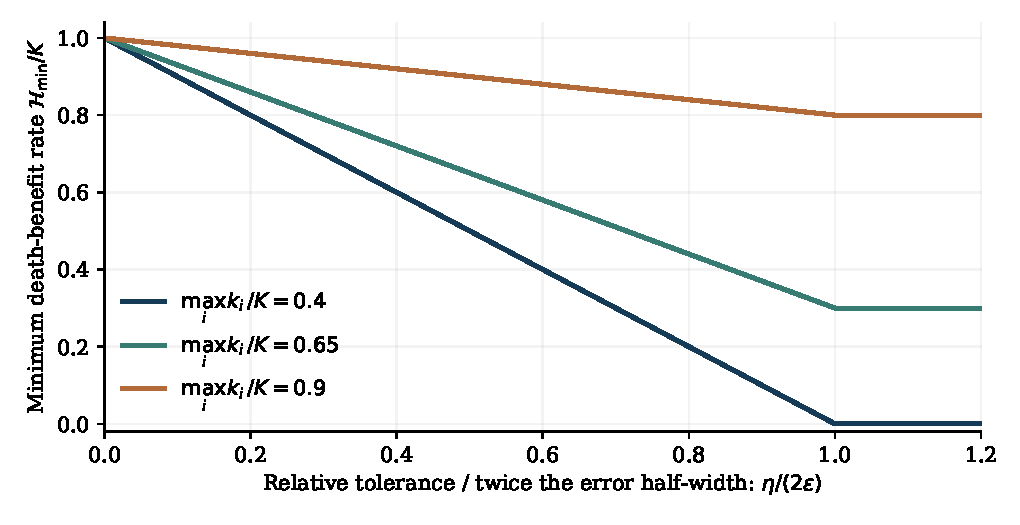
\includegraphics[width=.85\textwidth]{frontier.pdf}
\caption{Analytical robustness frontier under relative error tolerances. The normalized minimum death-benefit rate is $1-\rho+\rho(2s-1)_+$, where $s=\max_i k_i/K$ and $\rho=\min(1,\eta/(2\varepsilon))$. The figure displays a proved formula, not a Monte Carlo estimate.}\label{fig:frontier}
\end{figure}

\section{Exit Stopping Times and Information Asymmetry}\label{sec:exit}
\subsection{Public Valuation and Option Value}
Under correct intensities, $S_i(t)=A_i(t-)$ is a dynamically fair exit value. Theorem~\ref{thm:martingale} also applies to a public exit stopping time depending on account history. Exit may be valuable for liquidity or risk aversion even if it creates no additional expected wealth under linear present-value valuation. Expected-value neutrality therefore does not imply that the option is worthless to every investor.

Under unknown actual mortality, the true prospective reserve need not coincide with account value. For a specified continuation policy, the reserve is instead the account plus the expected discounted future misspecification drift. Paying the true reserve may require more than the existing individual account and would therefore require a separate funding arrangement. The account rule ensures funding; the robustness rule bounds the possible valuation discrepancy.

\begin{theorem}[Dynamic bound on misspecification-induced transfers]\label{thm:stop}
Consider a finite horizon $T$ and a member active at inception with account $A_i(0)$. Let $\sigma_i\le T$ be a $\calG$-stopping time, and put $\zeta_i=\sigma_i\wedge\tau_i$. Assume the compensated counting-process integrals are true martingales. At death, $H_i$ is paid; at exit, account value is paid. Then
\begin{equation}\label{eq:stopping}
J_i(\sigma_i)-A_i(0)
=\E\int_0^{\zeta_i}D(t)\Gamma_i(t)\,dt,
\end{equation}
where $J_i$ is the expected present value of all benefits to the member and estate. If the rule satisfies $|\Gamma_i(t)|\le\delta_i(t)$, then
\begin{equation}\label{eq:boundstop}
|J_i(\sigma_i)-A_i(0)|
\le\E\int_0^{\zeta_i}D(t)\delta_i(t)\,dt.
\end{equation}
\end{theorem}
\begin{proof}
The argument of Theorem~\ref{thm:martingale}, using the actual $\calG$-intensities, now produces drift $D(t)\Gamma_i(t)$. Subtracting its integral leaves a martingale. At $\zeta_i$, the account is fully settled through the death-benefit or exit payment. Taking expectations yields \eqref{eq:stopping}; the triangle inequality yields \eqref{eq:boundstop}.
\end{proof}
For $\delta_i(t)\le\bar\delta_i$, constant interest $r\ge0$ and $\sigma_i\le T$, the right-hand side is at most $\bar\delta_i(1-e^{-rT})/r$, with limit $\bar\delta_iT$ at $r=0$. This bound is uniform over stopping strategies. A pure option premium, defined as the advantage of optimal stopping over a specified continuation policy under the actual distribution, is a different object. If both policies lie within a common bound $R_i$ of $A_i(0)$, their present-value difference is at most $2R_i$. Neither bound gives a utility-based option value.

\subsection{Exogenous, Publicly Informed and Privately Informed Exits}
Exogenous exits without additional risk information are covered by Theorem~\ref{thm:martingale}. Publicly observed risk-profile changes can be handled prospectively by adjusting intensities. Private information may instead change the relevant intensity while the contractual rule remains unchanged. Theorem~\ref{thm:stop} bounds the effect only if intensities conditional on private information also lie within the agreed uncertainty set.

Without such a restriction, freely exercisable account-value exits cannot generally protect the pool. A simple counterexample is a one-period pool of two people contributing EUR~100 each: with equal probability, one receives EUR~200 and the other receives zero. If person 1 privately learns before settlement whether they will lose and may then withdraw EUR~100, the strategy ``exit if losing, otherwise remain'' has expected value EUR~150. Person 2 is left with an expected EUR~50. The initial public valuation was fair; the private signal makes the exit option financially valuable. This perfect signal explicitly lies outside a bounded relative-intensity uncertainty model.

Immediate exit and re-entry with the same capital and an unchanged publicly correct profile generate no additional expected gain under Theorem~\ref{thm:martingale}. New identities or account splitting must not create fictitious independent death risks. All accounts attached to the same insured life are aggregated for $k_i$, the capacity constraint and the death event. Otherwise, splitting could formally evade the concentration constraint while violating the assumption of separate death events.

\section{Payout Profiles and Remaining Trade-offs}\label{sec:income}
\subsection{Four Distinct Notions of Constancy}
Let $p_i(e_i,t)$ be survival probability from entry. Constancy of expected payout rates conditional on survival means
\[
\E[c_i(t)\mid\tau_i>t,\calF_{e_i}]=\bar c_i.
\]
The unconditional expected payout rate is then $p_i(e_i,t)\bar c_i$ and declines with survival probability. If the unconditional rate is instead required to be positive and constant, the survival-conditional rate must increase inversely with $p_i$. At $r=0$, a positive unconditional stream over an infinite horizon would also be impossible to finance with finite capital.

A constant future expected rate recalculated after every information update is a stronger dynamic requirement. Merely recalculating an annuity-based withdrawal rate does not establish it. Nominal and real constancy also differ through the price index: for a deterministic index $P(t)$, real constancy means constancy of $c_i(t)/P(t)$. With stochastic inflation, valuation in real units requires explicit investment and dependence assumptions.

\subsection{What an Annuity-Based Withdrawal Rule Actually Delivers}
For deterministic $\mu_i$ and $r$, define
\begin{equation}\label{eq:annuity}
a_i(t)=\int_t^\infty\exp\left(-\int_t^s[r(v)+\mu_i(v)]\,dv\right)ds,
\qquad c_i(t)=A_i(t)/a_i(t),
\end{equation}
where $a_i$ is finite and positive. Then $a_i'=(r+\mu_i)a_i-1$. Between events, $c_i$ has drift $-\mu_i c_i$. Deaths of other members contribute the additional expected rate $d_i/a_i$.

\begin{proposition}[Evolution of survival-conditional income]\label{prop:income}
Under correct deterministic intensities, independent death times, suitable integrability and no voluntary exit by the member considered, let
$m_i(t)=\E[c_i(t)\mid\tau_i>t,\calF_{e_i}]$. Then, almost everywhere,
\begin{equation}\label{eq:income}
m_i'(t)=-\E\left[\frac{k_i(t)-d_i(t)}{a_i(t)}\,\middle|\,\tau_i>t,\calF_{e_i}\right]
=-\E\left[\frac{\mu_i(t)H_i(t)}{a_i(t)}\,\middle|\,\tau_i>t,\calF_{e_i}\right]\le0.
\end{equation}
In particular, complete pooling throughout a time interval gives a constant survival-conditional expected rate on that interval. Exact constancy over the entire residual lifetime requires $H_i=0$ almost everywhere under the relevant conditional valuation.
\end{proposition}
\begin{proof}
The quotient rule and \eqref{eq:accountflow} give continuous drift $-\mu_i c_i$. For $Y_i(t)=\one_{\{\tau_i>t\}}c_i(t)$, the expectation drift is $\E[\one_{\{\tau_i>t\}}(-2\mu_i c_i+d_i/a_i)]$, because the member's own death additionally sets $c_i$ to zero. Using $p_i'=-\mu_i p_i$ and $m_i=\E[Y_i]/p_i$ yields \eqref{eq:income}. The integrand is nonnegative; a vanishing conditional expectation therefore implies that it vanishes almost surely.
\end{proof}
Exit by the member introduces an additional termination of payouts and selection effects. An expectation conditional on being ``alive and still active'' is not a substitute for an expectation conditional only on survival. The simulation reports these quantities separately.

The local frontier is directly related to the income profile. Let $g_i$ denote the expected drift of $c_i$ when the member's own death is suppressed for the survival-conditional calculation. Then
\[
g_i=-(k_i-d_i)/a_i,
\qquad \sum_i a_i(-g_i)=K-\sum_i d_i\ge\calH_{\min}.
\]
Thus the minimum death-benefit rate also bounds the weighted local decline of annuity-based payout rates from below under the reference model. This is a generator identity, not a statement about guaranteed individual income.

\subsection{The Last Survivor}
Without new entrants, a finite pool eventually has a last survivor. In a singleton state, $d_i=0$ and $H_i=A_i$. With constant $r$ and $\mu_i$, we have $a_i=1/(r+\mu_i)$, $A_i(t)=A_i(0)e^{-\mu_i t}$ and
\[
\E[c_i(t)\mid\tau_i>t]=c_i(0)e^{-\mu_i t}.
\]
The rate remains positive throughout life but is not constant. At $r=0$, a positive constant guaranteed rate $c$ would exceed capital on the event $\{\tau_i>A_i(0)/c\}$. At $r>0$, the fair constant life-annuity rate $c=(r+\mu_i)A_i(0)>rA_i(0)$ likewise cannot be financed on arbitrarily long survival paths. Constancy in expectation is not a guarantee; its failure for the present account rule follows separately from Proposition~\ref{prop:income}.

\section{Numerical Example and Reproducible Verification}\label{sec:numerics}
\subsection{A State Attaining the Bound}
Three accounts each contain EUR~100,000, with $\mu=(0.01,0.02,0.03)$. Thus $k=(1000,2000,3000)$ and $K=6000$. Complete nominal pooling is possible. For $\varepsilon=0.2$ and relative error tolerance $\eta=0.1$, we obtain $\rho=0.25$ and
\[
d^*=(250,500,750),\qquad
F=\begin{pmatrix}0&0&250\\0&0&500\\250&500&0\end{pmatrix}.
\]
Each death transfers EUR~25,000 to other members and EUR~75,000 to the estate. On the death of member 3, members 1 and 2 receive $250/0.03=8333.33$ and $500/0.03=16666.67$ euros, respectively. The modelled death-benefit rate is EUR~4,500 per year. For $z=(0.8,0.8,1.2)$,
\[
\Gamma=(100,200,-300),\qquad 2\varepsilon d=(100,200,300).
\]
All individual absolute bounds are attained in this state. The 10\% tolerance is relative to annual mortality exposure, not to total account value or income.

\subsection{Numerical Design}
The accompanying script \texttt{robust\_tontine.R} uses Base R only. It checks 180 randomly generated states with $n\in\{1,2,3,5,10,20\}$, highly heterogeneous lognormally generated exposures and error tolerances. The checks cover balance, symmetry of the construction, zero diagonal, nonnegativity, capacities and the frontier formula. For $n\le5$, every vertex of the uncertainty box is evaluated and compared with Lemma~\ref{lem:worst}. These checks do not replace the proofs.

Dynamic verification comprises five scenarios with 10,000 independent paths each and fixed seed 20261002. We use $r=0.02$, a horizon of $T=20$ years, ages 55, 70 and 85, and contributions of EUR~10,000, EUR~100,000 and EUR~1,000,000. Individual intensity is parameterized by $\mu(x)=0.008\exp(0.09(x-65))$ and subsequently held constant throughout simulated membership. This is a deliberately simple, non-empirically calibrated model check; it does not implement Gompertz ageing along each path.

Closed scenarios start with three members. Open scenarios add three members in each of years 2, 4 and 6. Exogenous exits have intensity 0.08. The misspecification scenario uses $z=(0.8,0.8,1.2)$ in each entry cohort and the robust rule with $\varepsilon=0.2$ and $\eta=0.1$. A singleton scenario tests the last-survivor case. Optimal private-information exit strategies are not solved numerically.

Death, exit and entry times are processed in an event-driven simulation. Between events, $A_i(t+h)=A_i(t)e^{-\mu_i h}$ and running benefits are integrated analytically in present-value terms. Before every death, the rule is recalculated from current accounts. The remaining account is explicitly paid out at horizon $T$. This verifies the finite-horizon valuation identity including terminal capital; the results are not interpreted as establishing lifetime fairness without residual assets.

Individual present values are measured at each member's entry date. For aggregate results, contributions and benefits are consistently discounted to time zero. Mixing entry-date valuations would produce an incorrect balance, particularly in the open pool. Standard errors are calculated from independent path observations. For conditional payout rates, the effective sample size is the number of surviving or active members, respectively, rather than 10,000. Intervals are normal Monte Carlo intervals; simultaneous coverage is not claimed.

\subsection{Results}
\begin{table}[htbp]\centering\small
\caption{Selected individual present-value ratios. All benefits, including estate, exit and terminal-account payments, are compared with capital at entry. Intervals quantify Monte Carlo uncertainty.}
\begin{tabular}{llrrr}\toprule
Scenario & Member & PV / capital & Standard error & 95\% interval\\\midrule
Closed, nominal & 1 & 0.9967 & 0.0022 & $[0.9924;1.0010]$\\
Closed, nominal & 2 & 0.9977 & 0.0034 & $[0.9910;1.0045]$\\
Closed, nominal & 3 & 1.0003 & 0.0003 & $[0.9996;1.0009]$\\
Closed, robust & 1 & 1.0000 & 0.0005 & $[0.9990;1.0010]$\\
Closed, robust & 2 & 0.9989 & 0.0009 & $[0.9973;1.0006]$\\
Closed, robust & 3 & 1.0001 & 0.0001 & $[0.9999;1.0003]$\\
Open with exits & 1 & 0.9974 & 0.0017 & $[0.9941;1.0007]$\\
Open with exits & 2 & 0.9983 & 0.0033 & $[0.9917;1.0048]$\\
Open with exits & 3 & 0.9978 & 0.0046 & $[0.9889;1.0067]$\\
Open, robust, error & 1 & 1.0026 & 0.0004 & $[1.0020;1.0033]$\\
Open, robust, error & 2 & 1.0087 & 0.0007 & $[1.0072;1.0101]$\\
Open, robust, error & 3 & 0.9995 & 0.0011 & $[0.9973;1.0018]$\\
Singleton & 1 & 1.0000 & 0.0000 & $[1.0000;1.0000]$\\
\bottomrule\end{tabular}\end{table}
\begin{table}[htbp]\centering\small
\caption{Payout rate after five years relative to its value at entry, conditional only on survival. These closed scenarios have no exits.}
\begin{tabular}{llrrr}\toprule
Scenario & Member & Expected rate & Standard error & Survivors\\\midrule
Nominal & 1 & 1.0000 & 0.0004 & 9828\\
Nominal & 2 & 0.9930 & 0.0010 & 9382\\
Nominal & 3 & 0.7906 & 0.0002 & 7808\\
Robust & 1 & 0.9878 & 0.0001 & 9839\\
Robust & 2 & 0.9522 & 0.0003 & 9366\\
Robust & 3 & 0.7865 & 0.0001 & 7868\\
Singleton & 1 & 0.9392 & 0.0000 & 9421\\
\bottomrule\end{tabular}\end{table}
\begin{table}[htbp]\centering\small
\caption{Misspecification and integrated tolerance for the first entry cohort in the open robust scenario. The relative error half-width is 20\%, and the relative annual error tolerance is 10\%.}
\begin{tabular}{rrrr}\toprule
Member & PV / capital minus 1 & Standard error & Expected bound / capital\\\midrule
1 & 0.0026 & 0.0004 & 0.0027\\
2 & 0.0087 & 0.0007 & 0.0095\\
3 & -0.0005 & 0.0011 & 0.0240\\
\bottomrule\end{tabular}\end{table}
The maximum relative error in the R state checks was $2.17\cdot10^{-16}$, that in the 180 independent linear optimization checks was $3.72\cdot10^{-16}$. The maximum relative dynamic balance error was $1.68\cdot10^{-15}$. The immediate change in other accounts at entry and exit was exactly zero. The aggregate present-value ratio, consistently discounted to time zero, was one on every path in all scenarios, up to rounding error; its Monte Carlo standard error is therefore merely a numerical rounding measure. Individual members, in contrast, have stochastic individual present values.

Account and balance checks confirm pathwise funding up to rounding error. Simulations with correct intensities test the finite-horizon fairness identity, whereas the misspecification scenario illustrates possible individual shifts with a balanced aggregate budget. For each member in that scenario, the pathwise integrated error tolerance is also calculated and averaged. A finite Monte Carlo sample need not satisfy an expectation bound exactly; results must be interpreted together with their standard errors.

For the singleton, the analytical payout rate conditional on survival after five years is $\exp(-5\mu(70))$ times the initial rate. The Monte Carlo check reproduces this quantity without payout dispersion among survivors, since their account path is deterministic in this case. In particular, an annuity-based withdrawal rule alone does not produce constant survival-conditional income.

\section{Extensions and Limitations}
\paragraph{Capital markets.} If accounts are carried at the actual common portfolio value and benefits are financed from them, the budget identity remains valid. However, expected-present-value fairness under the physical measure does not automatically follow from discounting risky returns at the risk-free rate. The mortality drift remains identifiable, but return drift and possibly a different valuation measure must also be considered. A complete capital-market optimization is outside the stated theorems.

\paragraph{Systematic longevity.} An unknown common proportional factor preserves local fairness of balanced mortality transfers. Different cohort sensitivities instead generate relative errors and hence $\Gamma\ne0$. Correlation alone is insufficient for robustness. Common death events would require additional jump-allocation rules and are excluded.

\paragraph{Costs.} Administration costs must be paid from existing accounts or agreed separately. Fairness then concerns benefits plus transparently allocated costs, and need not hold for net retirement income alone. Entry costs must not be implicitly transferred to existing members.

\paragraph{Uncertainty sets.} The rectangular set yields a simple sharp formula. For a general set $\mathcal U$, the exact identity is
\[
\sup_{u\in\mathcal U}|\Gamma_i|
=\max\{h_{\mathcal U}(F_{i\cdot}-d_ie_i),
         h_{\mathcal U}(-F_{i\cdot}+d_ie_i)\},
\]
where $h_{\mathcal U}$ denotes the support function, $F_{i\cdot}$ the row vector, and $e_i$ the unit vector in this display. With different individual error widths, admissible counterparties matter, and a scalar capacity reduction may no longer suffice. A common relative error half-width is therefore a substantive assumption of the closed-form main result.

\paragraph{Further optimization.} The exposure vector maximizing pooling is unique, but $F$ need not be. Among attaining matrices, secondary objectives could minimize variance, concentration of individual credits or discontinuity at transactions. This is an open follow-up problem. The optimal joint choice of $\delta_i$, consumption and exit strategy under risk aversion is also open. These utility and risk objectives are not presented as solved.

\section{Conclusion}
An open heterogeneous tontine can be fully funded through individual accounts and balanced death-contingent transfers, and dynamically fair under correct public mortality information. Exits at account value preserve the immediate accounts and nominal expected total present values of remaining members. They do not automatically preserve future distributions or risk burdens.

The main theorem quantifies the adjustment required by unknown individual mortality: an admissible error budget reduces poolable exposure to $b_i$, and finite concentration further restricts it to $\min(b_i,B-b_i)$. The minimum necessary modelled death-benefit rate is exactly $K-B+(2\max_i b_i-B)_+$. Complete robust local fairness against independently variable individual errors requires eliminating mortality transfers. Bounded fairness errors instead permit a transparently determined pooling fraction.

The simplest viable construction combines exits at account value, a common relative error tolerance and the explicit maximal coupling rule. It provides openness, heterogeneity, pathwise funding and model-dependent individual fairness for total benefits. Private information is quantitatively bounded only within the specified intensity uncertainty. Globally constant expected income conditional on survival, fairness of survival benefits alone and unchanged risk after exits are not unconditional properties of this construction.

\appendix
\section{Reproduction and Review of the Working Paper}
All numerical results in this version are generated by
\begin{verbatim}
Rscript robust_tontine.R 10000 results
python3 validate_frontier.py
python3 build_results.py
pdflatex manuscript.tex
bibtex manuscript
pdflatex manuscript.tex
pdflatex manuscript.tex
\end{verbatim}
The Python steps require NumPy, SciPy, Pandas and Matplotlib; the R script requires no add-on packages. The Python validation script solves independent linear optimization problems, whereas the R script checks the explicit coupling and event-driven dynamics. CSV files and R session information are included.

The main formula, the energy identity and the stopping-time bound are proved under their stated assumptions. Numerical results are model checks. Priority of the combined contribution remains an unverified research claim. Before submission, independent mathematical review, a full-text comparison with relevant transfer and surrender-value papers, and decisions on authorship and the applicable disclosure requirements for AI assistance are required.

\bibliographystyle{plainnat}
\bibliography{references}
\end{document}
